\section {Experimentálne meranie hustoty stavov v disorderovanom kove}
V tejto kapitole predstavíme experimentálnu metódu merania hustoty stavov
Táto metóda využíva efekt tunelovania elektrónu cez potenciálovú bariéru.

Experimentálna sústava pozostáva z dvoch kovov odelených izolantom. Naľavo máme čistý 
kov, ktorého hustotu poznáme - {\it známy kov}. Napravo máme disorderovaný kov, ktorého 
hustotu stavov budeme merať - {\it skúmaný kov}. Izolant tvorí potenciálovú bariéru.
Na sústavu priložíme napätie  $U$ a budeme merať prúd.  

Bez priloženého napätia ($U=0$) popisuje Hamiltonián 
\begin{equation}
 \label{eq:02barrier}
 \hat{H}=\frac{\hbar^2 \laplace }{2m}+V(x) \text{,}
\end{equation} 
kde 
\begin{equation}
 \label{eq:02potential_barrier}
 V(x)=
 \begin{cases}
    V_0,& \text{pre } 0<x<b\\
    0,              & \text{inak}
\end{cases}\text{,}
\end{equation} 
kde $b$ je šírka bariéry,

Hladanie vlastných stavov Hamiltoniánu \eqref{eq:02barrier} je učebnicový problém, ktorý sa 
štandartne rieši nájdením vlnových funkcii v troch oblastiach a následným ,,zošívaním'' 
pomocou podmienky spojitosti vlnovej funkcie a jej derivácie. 

Štandartný spôsob riešenia však zlyhá po priložení napätia na experimentálnu sústavu. 
Preto predstavíme iný spôsob.

Majme teraz dve nekonečne široké bariéry z ľava:
\begin{equation}
 \label{eq:02potential_left}
 V_l(x)=
 \begin{cases}
    V_0,& \text{pre } 0<x\\
    0,              & \text{inak}
\end{cases}\text{,}
\end{equation}
a podobne sprava
 \begin{equation}
 \label{eq:02potential_right}
 V_r(x)=
 \begin{cases}
    V_0,& \text{pre } b>x\\
    0,              & \text{inak}
\end{cases}\text{.}
\end{equation}
Pre obe bariéry \eqref{eq:02potential_left} a \eqref{eq:02potential_right} vieme určiť 
vlastné stavy $\psi_{l}(x)$ a $\psi_{r}(x)$. Tieto stavy sú očividne dobrou aproximáciou 
stavov naľavo a napravo od konečnej bariéry \eqref{eq:02potential_barrier}. Nie sú to však 
vlastné stavy hamiltoniánu \eqref{eq:02barrier}, preto musíme riešiť časovú SchR 
\begin{equation}
 \label{eq:02time_schr}
 i\hbar \frac{d}{dt}\psi(x,t)=\hat{H} \psi(x,t)\text{.}
\end{equation} 
Časticu je v čase $t=0$ na ľavo od bariéry teda v stave $\psi_l(x)$, teda máme počiatočnú 
podmienku 
\begin{equation}
 \label{eq:02init_cond} 
 \psi(x,0)=\psi_l(x)\text{.}
\end{equation}
Riešenie časovej SchR \eqref{eq:02time_schr} hľadáme v tvare:
\begin{equation}
 \label{eq:02time_schr_solution}
 \psi(x,t)=c_l(t)\psi_l(x)e^{-\frac{iE_l t}{\hbar}}+\sum_{\forall r} c_r(t)\psi_l(x)e^{-\frac{iE_r t}
{\hbar}}\text{,}
\end{equation}  
kde s počiatočných podmienok \eqref{eq:02init_cond} dostávame:
\begin{equation}
 \label{eq:02time_schr_coeficients} 
c_l(0)=1 , c_r(0)=0 \text{.}
 \end{equation} 
 Pre slabo preniknuteľnú bariéru vieme koeficienty aproximovať ako:
 \begin{equation}
 \label{eq:02time_schr_coeficients_approx} 
c_l(t)\doteq1,c_l'(t)\doteq1 , c_r(t)\doteq0 \text{.}
 \end{equation} 
 
Dosadením \eqref{eq:02time_schr_solution}  do \eqref{eq:02time_schr} a použitím 
\eqref{eq:02time_schr_coeficients_approx} 
a následnými úpravami  dostávame
\begin{equation}
 \label{eq:02golden_rule}
 w_{r\to l}=\frac{2\pi}{\hbar} \bra{\psi_l}H-E_l\ket{\psi_r}\delta(E_l-E_r)\text{.}
\end{equation} 
Dostali sme vzťah podobný Fermiho zlatému pravidlu, ktorý popisuje pravdepodobnost 
prechod zo stavu $\psi_l$  do stavu $\psi_r$. 

V ďalšom zavedieme označenie
\begin{equation}
\label{eq:02t}
t_{k_l \to k_r}=\bra{\psi_l}H-E_l\ket{\psi_r}
\end{equation}

Teraz priložíme na sústavu napätie $U$, čo spôsobí zmenu dna energetického pásu na 
pravej strane bariéry $\Delta E_c$.  Potenciálová bariéra má teraz tvar lineárnej funkcie.
Obsadzovacie čísla jednotlivých elektrónových stavov budú na ľavo dané Fermi-Diracovým rozdelením:
\begin{equation}
 \label{eq:02fermidirac_left}
 f_l(k_l)=\frac{1}{e^{\frac{E_{k_l}-\mu_l}{k_bT}}+1}\text{,}
\end{equation} 

podobne pre stavy na pravo:

\begin{equation}
 \label{eq:02fermidirac_right}
 f_r(k_r)=\frac{1}{e^{\frac{E_{k_r}-\mu_r}{k_bT}}+1}\text{.}
\end{equation} 

Počet elektrónov ktoré prejdu zľava do prava, resp sprava do ľava.
\begin{equation}
\label{eq:02elctronsLTR}
\Gamma^+(\Delta E)=\sum_{k_l}{\sum_{k_r} w_{k_l \to k_r} f_l(k_l)[1-f_r(k_r)]}
\end{equation}

\begin{equation}
\label{eq:02elctronsRTL}
\Gamma^-(\Delta E)=\sum_{k_l}{\sum_{k_r} w_{k_r \to k_l} f_r(k_r)[1-f_l(k_l)]}
\end{equation}

Kde $\Delta E$ je rozdiel energii medzi stavmi naľavo a napravo, pozri obrázok. Celkový prúd je teda 
\begin{equation}
\label{eq:02current}
I={\Gamma^+(\Delta E) - \Gamma^-(\Delta E)}
\end{equation}


V roviniciach \eqref{eq:02elctronsLTR} a \eqref{eq:02elctronsRTL}  prejdeme od sumy k integrálu a dosadíme Zlaté pravidlo \eqref{eq:02golden_rule}. Nakoniec prejdeme k integrálu cez energiu, kde musíme násobiť hustotu stavov.
\begin{align*}
\Gamma^+(\Delta E)=\frac{2\pi}{\hbar}2\sum_{k_l} \sum_{k_r} {|t_{k_l \to k_r}|^2f_l(k_l)[1-f_r(k_r)]\delta(E_{l}-E_{r})}= \\
\frac{2\pi}{\hbar}2 \int_{0}^{\infty}\frac{L}{\pi} dk_{r}\int_{0}^{\infty}\frac{L}{\pi} dl_{l} {|t_{k_l \to k_r}|^2f_l(k_l)[1-f_r(k_r)]\delta(E_{l}-E_{r})} \simeq\\
 \frac{2\pi}{\hbar}2 |t|^2 \int_{E_{c,l}}^{\infty}\frac{L}{\pi}\rho_r(E_r)dE_r\int_{E_{c,r}}^{\infty}\frac{L}{\pi} N_r(E_r)dE_r {f_l(k_l)[1-f_r(k_r)]\delta(E_{l}-E_{r})} \text{,}\\
\end{align*}
kde sme v poslednom riadku zanedbali závislosť transmisného koeficientu $t(k_l,k_r)$ . Podobným spôsobom vieme upraviť aj vzťah \eqref{eq:02elctronsRTL}.
Takto upravené vzťahy dosadíme do rovnice pre celkový prúd prechádzajúci sústavou \eqref{eq:02current} a dostaneme 
\begin{equation}
\label{eq:02current2}
I=e\frac{4\pi|t|^2}{\hbar}\int_{E_{cl}}^\infty dE_l\rho_l(E_l)\rho_r(E_l)(f_l(E_l)-f_r(E_l)) \text{,}
\end{equation}
kde sme navyše využili $\delta$-funkciu a zbavili sa integrovania cez $E_r$. 


V limite nízkych teplôt $T \simeq 0$ Fermi-Diracove funkcie prejdú na $\Theta$-funkcie. Preto dostávame
\begin{align}
I=e\frac{4\pi|t|^2}{\hbar}[\int_{E_{cl}}^{\mu_l}dE_l-\int_{E_{cl}}^{\mu_r}dE_l\rho_r(E_l)\rho_l(E_l)]\text{,}
\end{align}
Chemické potenciály na ľavej a pravej strane bariéry $\mu_r$ a $\mu_l$ sa líšia o $-Ue$ teda integrál napíšeme ako
\begin{align}
\label{eq:02current3}
I = e \frac{4\pi|t|^2}{\hbar}\int_{\mu_r}^{\mu_r-Ue}dE_l\rho_r(E_l)\rho_l(E_l)\text{.}
\end{align}
 Na ľavej strane bariéry je známy kov bez disorderu. Jeho hustota stavov sa v okolí Fermiho energie dá aproximovať konštantou. Fermiho energia (a teda aj chemický potenciál naľavo $\mu_l$ i napravo $\mu_r$ )je rádovo $E_F\sim\SI{10}{\eV}$ a rozdiel enregí je rádovo $eU\sim \SI{100}{\milli\eV}$, teda na celom intervale integrálu v
\eqref{eq:02current3} možno nahradiť hustotu stavov $\rho_l(E_l)$ konštantou $\rho_1(\mu_l)$, čiže hustotou stavov na Fermiho hladine. Konštantu vyjmeme pred integrál a dostaneme
\begin{align}
I = e \frac{4\pi|t|^2}{\hbar}\rho_l(\mu_l)\int_{\mu_r}^{\mu_r-Ue}dE_l\rho_r(E_l)\text{,}
\end{align}
teda pre diferenciálnu vodivosť dostaneme
\begin{align}
\label{eq:02diff}
\frac{d I}{d U}=e\frac{4\pi|t|^2}{\hbar}\rho_l(\mu_l)\rho_r(\mu_r-Ue)
\end{align}
Diferenciálnu vodivosť vieme experimentálne merať, a to určením voltampérovej charakteristiky. Preto z \eqref{eq:02diff} vyjaderíme jedinú neznámu veličinu, hustotu stavov skúmaného kovu napravo. Dostaneme priamu úmernosť medzi difernciálnou vodivosťou a hustotou stacvov 
\begin{align}
\rho_r(\mu_r-Ue)=\alpha \frac{d I}{d U} \text{,}
\end{align}
kde $\alpha=\frac{\hbar}{4\pi|t|^2e}$ je konštanta úmernosti. 

Hustotu stavov meriame určením voltampérovej charakteristiky sústavy {\it známy} kov - bariéra (izolant) - {\it skúmaný} kov, ktorá je po prenásobení konštantou $\alpha$ hustota stavov. {\it Známy} kov musí byť čistý (bez disorderu) aby sme v okolí Fermiho energie mohli použiť parabolický disperzný zákon a týmpádom aproximáciu $\rho_l(E_l)\approx\rho_l(\mu_l)$. 

Pri meraní vložíme najskôr na obe strany čistý kov, a určíme jeho diferenciálnu vodivosť, ktorú označíme  $G_0(U)$. Potom meriame diferenciálnu vodivosť sústavy s disorderovaným kovom napravo $G(U)=\frac{dI(U)}{dU}$. 

Pre hustotu stavov skúmaného kovu dostaneme:
\begin{align}
\frac{\rho_r(E)}{\rho_l(E_F)} = \frac{G(U)}{G_0(U)}
\end{align}

Kde $\rho_l(E_F)$ je daná parabolickým disperzným zákonom.
\begin{figure}[H]
\centering
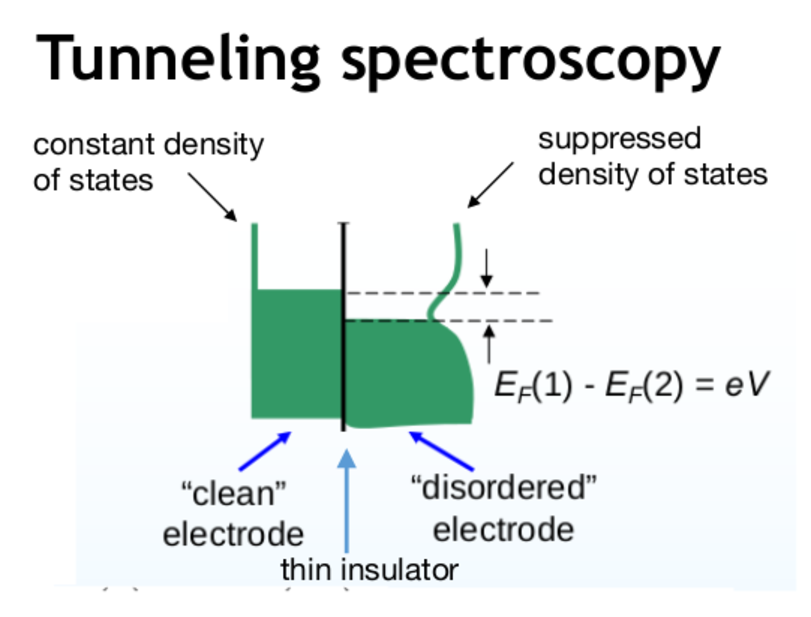
\includegraphics[scale=1]{grafy/DOS-cropped}
\caption{Meranie hustoty stavov tunelovou spektroskopiou. V experimente máme "čistý" a "disorderovaný" kov oddelené tenkou vrstvou izolantu. Meraná veličina je difernciálna vodivosť $\frac{d I}{d U}$}. 
\end{figure}
\begin{figure}[H]
\centering
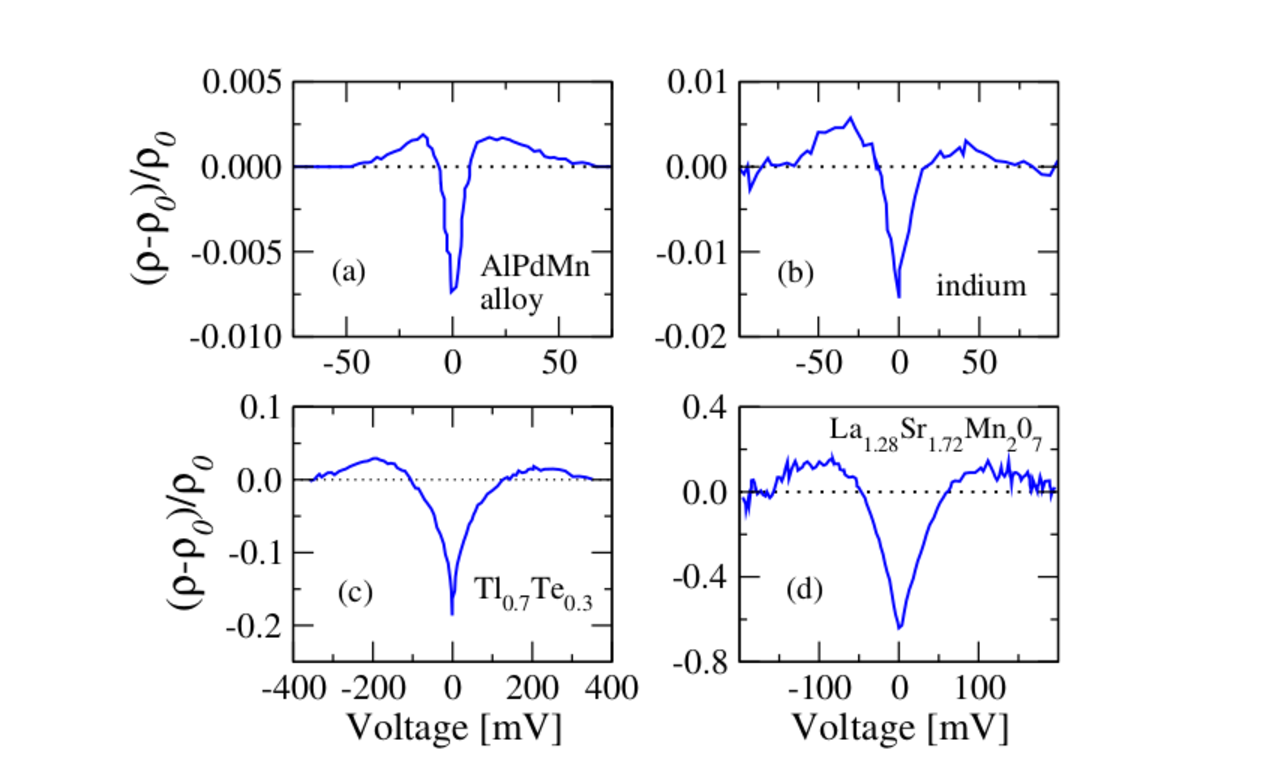
\includegraphics[scale=1]{grafy/B2}
\caption{Výsledky merania hustoty stavov tunelovou spektroskopiou pre rôzne zliatiny. Vo výsledných grafoch môžme vidieť pokles hustoty stavov v okolí Fermiho Energie, podľa predpovedí Altschulera-Aronova. Zároveň vidíme  nárast hustoty stavov v oblasti ďalej od $E_F$.}
\end{figure}